\documentclass[12pt,a4paper]{article}
\usepackage[T1]{fontenc}
\usepackage[utf8]{inputenc}
\usepackage{times}
\linespread{1.5}
\usepackage[version=3]{mhchem}
\usepackage{amsmath}
%\usepackage{biblatex}
\usepackage{SIunits}
\usepackage[estonian]{babel}
\usepackage{parskip}
\usepackage{graphicx}
\usepackage{float}
\usepackage{hyperref}
\usepackage{fullpage}
\usepackage[firstinits=true,abbreviate=false,sorting=none,backend=bibtex]{biblatex}
\usepackage[labelfont={bf,small},textfont={small,it},width=0.8\textwidth]{caption}
\usepackage{subcaption}
\usepackage{pdfpages}
\usepackage[nonumberlist]{glossaries}
\makeglossaries
\usepackage{imakeidx}
\makeindex
\usepackage[title,titletoc]{appendix}
\usepackage{breakurl}
\input{glyphtounicode}
\pdfgentounicode=1

%\captionsetup{}{}

\renewcommand*{\multinamedelim}{\addcomma\space}
\renewcommand*{\finalnamedelim}{\addcomma\space}

\renewcommand*{\newunitpunct}{\addcomma\space}

\DeclareFieldFormat*{title}{#1}
\DeclareFieldFormat{journaltitle}{#1}

\renewbibmacro{in:}{%
  \ifentrytype{article}{%
  }{%
    \printtext{\bibstring{in}\intitlepunct}%
  }%
}

\renewbibmacro*{volume+number+eid}{%
  \printfield{volume}%
  \setunit*{\addnbspace}%
  \printfield{number}%
  \setunit{\addcomma\space}%
  \printfield{eid}}
\DeclareFieldFormat[article]{number}{\mkbibparens{#1}}

\renewcommand*{\bibpagespunct}{\addspace}

\DeclareFieldFormat{pages}{#1}

\renewbibmacro*{publisher+location+date}{%
  \printlist{publisher}%
  \setunit*{\addcomma\space}%
  \printlist{location}%
  \setunit*{\addcomma\space}%
  \usebibmacro{date}%
  \newunit}

\AtBeginDocument{\renewcommand\refname{Kasutatud kirjandus}}
\AtBeginDocument{\renewcommand{\contentsname}{Sisukord}}
\AtBeginDocument{\renewcommand{\glossaryname}{Lühendid}}
\renewcommand*{\glspostdescription}{}

\bibliography{library}
%
% glossary.tex
%
% Fail lühendite/akronüümide ja mõistete defineerimiseks.
% Tekstis kasutatud mõisted ilmuvad automaatselt eraldi leheküljele 
% mõistete selgitusse.
%
% Kasutamine:
%   \gls{} - väikese algustähega mõiste/lühend. Lühendi puhul ilmub esimesel
%            korral teksti:
%               tähendus (LHND)
%            Edasisel kasutamisel tekitab see ainult lühendi.
%   \Gls{} - samasugune nagu \gls{}, suure algustähega
%   \glspl{}, \Glspl{} - mitmuse vormid eelnevatest
%

% Akronüüm koos nii lühendi kui ka selle tähenduse mitmustega
\newacronym[\glsshortpluralkey={KTA-d},longplural=kolmetähelised akronüümid]{kta}{KTA}{kolmetäheline akronüüm}

% Lihtsalt akronüüm ilma mitmusteta
\newacronym{aim}{AIM}{akronüüm ilma mitmuseta}

% Tavaline mõiste
\newglossaryentry{tavaline}
{
  name=tavaline mõiste,
  description={tavalise mõiste veel tavalisem seletus}
}

\title{Tartu Ülikooli bakalaureusetöö}

\author{Hendrik Kaju}
\begin{document}

  % Impordime tiitellehe
	\begin{titlepage}
\begin{center}

\textsc{Tartu Ülikool}\\
\textsc{Loodus- ja tehnoloogiateaduskond}\\
\textsc{Keemia Instituut}\\[3.5cm]

{\large\textsc{Autor}}\\[0.2cm]
{\Large
\textsc{\bfseries 
Pealkiri}}\\[0.2cm]
\textsc{Bakalaureusetöö (12 EAP)}\\[3.2cm]

\begin{flushright} 
\emph{Juhendaja:} \\
\textsc{Juhendaja}
\end{flushright}

\vspace{3cm}
\begin{flushleft} 
\emph{Kaitsmisele lubatud:}\\[0.5cm]
\emph{Juhendaja: ....................................................}\\[0.5cm]
\emph{Juhendaja: ....................................................}\\
\end{flushleft}

%\vfill
\vspace{1.5cm}
% Bottom of the page
\textsc{Tartu 2013}%\\[0.1cm]

\end{center}
\end{titlepage}
	
	% Eemaldame leheküljenumbri?
  \thispagestyle{empty}
	
  \clearpage
  \pagestyle{plain}
  % 
  \tableofcontents

	\clearpage
	\printglossaries
	\addcontentsline{toc}{section}{Lühendid}
	
	%
% introduction.tex
%
% Sissejuhatus
%

\section{Sissejuhatus}

\subsection{Mis see on?}

Tegemist on 2013. aastal Keemia Instituudis kaitstud bakalaureusetöö vormistusnäidisega.
Kui ma hakkasin tööd kirjutama, ei leidnud ma ühtegi terviklikku LaTeXis vormistatud lõputöö näidist ja pidin seetõttu otsast peale alustama.
Loodetavasti on tulevastel LaTeXi-huvilistel töökirjutamine/vormistamine veidi lihtsam.

\subsection{Kasutamine}
Tööga on kaasas `Rakefile`, mis lihtsustab mõnevõrra kompileerimist.
Selle kasutamiseks peab olema paigaldatud Ruby ja `rake`.

\begin{verbatim}
    gem install rake
\end{verbatim}

\LaTeX-i failide kompileerimiseks saad kasutada käsku `rake compile` ja 
töökataloogi puhastamiseks ajutistest failidest `rake clean`.
Tulemus on failis `thesis.pdf`.

\subsection{Struktuur}

Põhifail on `thesis.tex`.
Tiitelleht ja kõik peatükid on eraldi failides.
Failid on võimaluste piires kommenteeritud.

\subsection{Litsents}

Töö on avaldatud MITi litsentsi all.
Täpsemalt saab lugeda failist `LICENSE`.
	
  %
% overview.tex
%
% Kirjanduse ülevaade
%

\section{Valdkonna ülevaade}

\subsection{Lühendid ja mõisted}

\Gls{tavaline} on mõiste, mis ilmub pärast teksti lisamist automaatselt ka mõistete leheküljele.
\Gls{aim} on tavaline akronüüm.
\Gls{aim}i teistkordsel kasutamisel ilmub teksti ainult lühend.
\Glspl{kta} on akronüümid, mille jaoks on defineeritud ka mitmus.

\subsection{Valemid}

Valemeid saab kasutada nii teksti sees ($ I = I_0 \cdot \textrm{exp}(-\epsilon l c)$) kui ka eraldiseisvalt:

\begin{equation}
    \label{gauss}
    \nabla\cdot{\bf D} = \rho
\end{equation}
\begin{equation}
    \label{gaussmagnet}
    \nabla\cdot{\bf B} = 0
\end{equation}
\[
    \nabla\times{\bf E} = - {{\partial{\bf B}}\over{\partial t}}
\]
\[
    \nabla\times{\bf H} = {\bf J} + {{\partial{\bf D}}\over{\partial t}}
\]

\subsection{Tabelid}

\begin{table}[H]
    \caption{\label{tabel}Tabel huvitavate numbritega}
    \centering
    \begin{tabular}{c|c|c}
    Number & Esimene arv & Teine arv \\
    \hline
    1 & 123 & 456 \\
    2 & 789 & 101112 \\
    3 & 131415 & 161718 \\
    4 & 192021 & 222324 \\
    5 & 252627 & 282930 \\
    \hline
    \multicolumn{3}{l}{Väike seletustekst tabeli lõppu}
    \end{tabular}
\end{table}

\subsection{Joonised}

\begin{figure}[H]
    \centering
    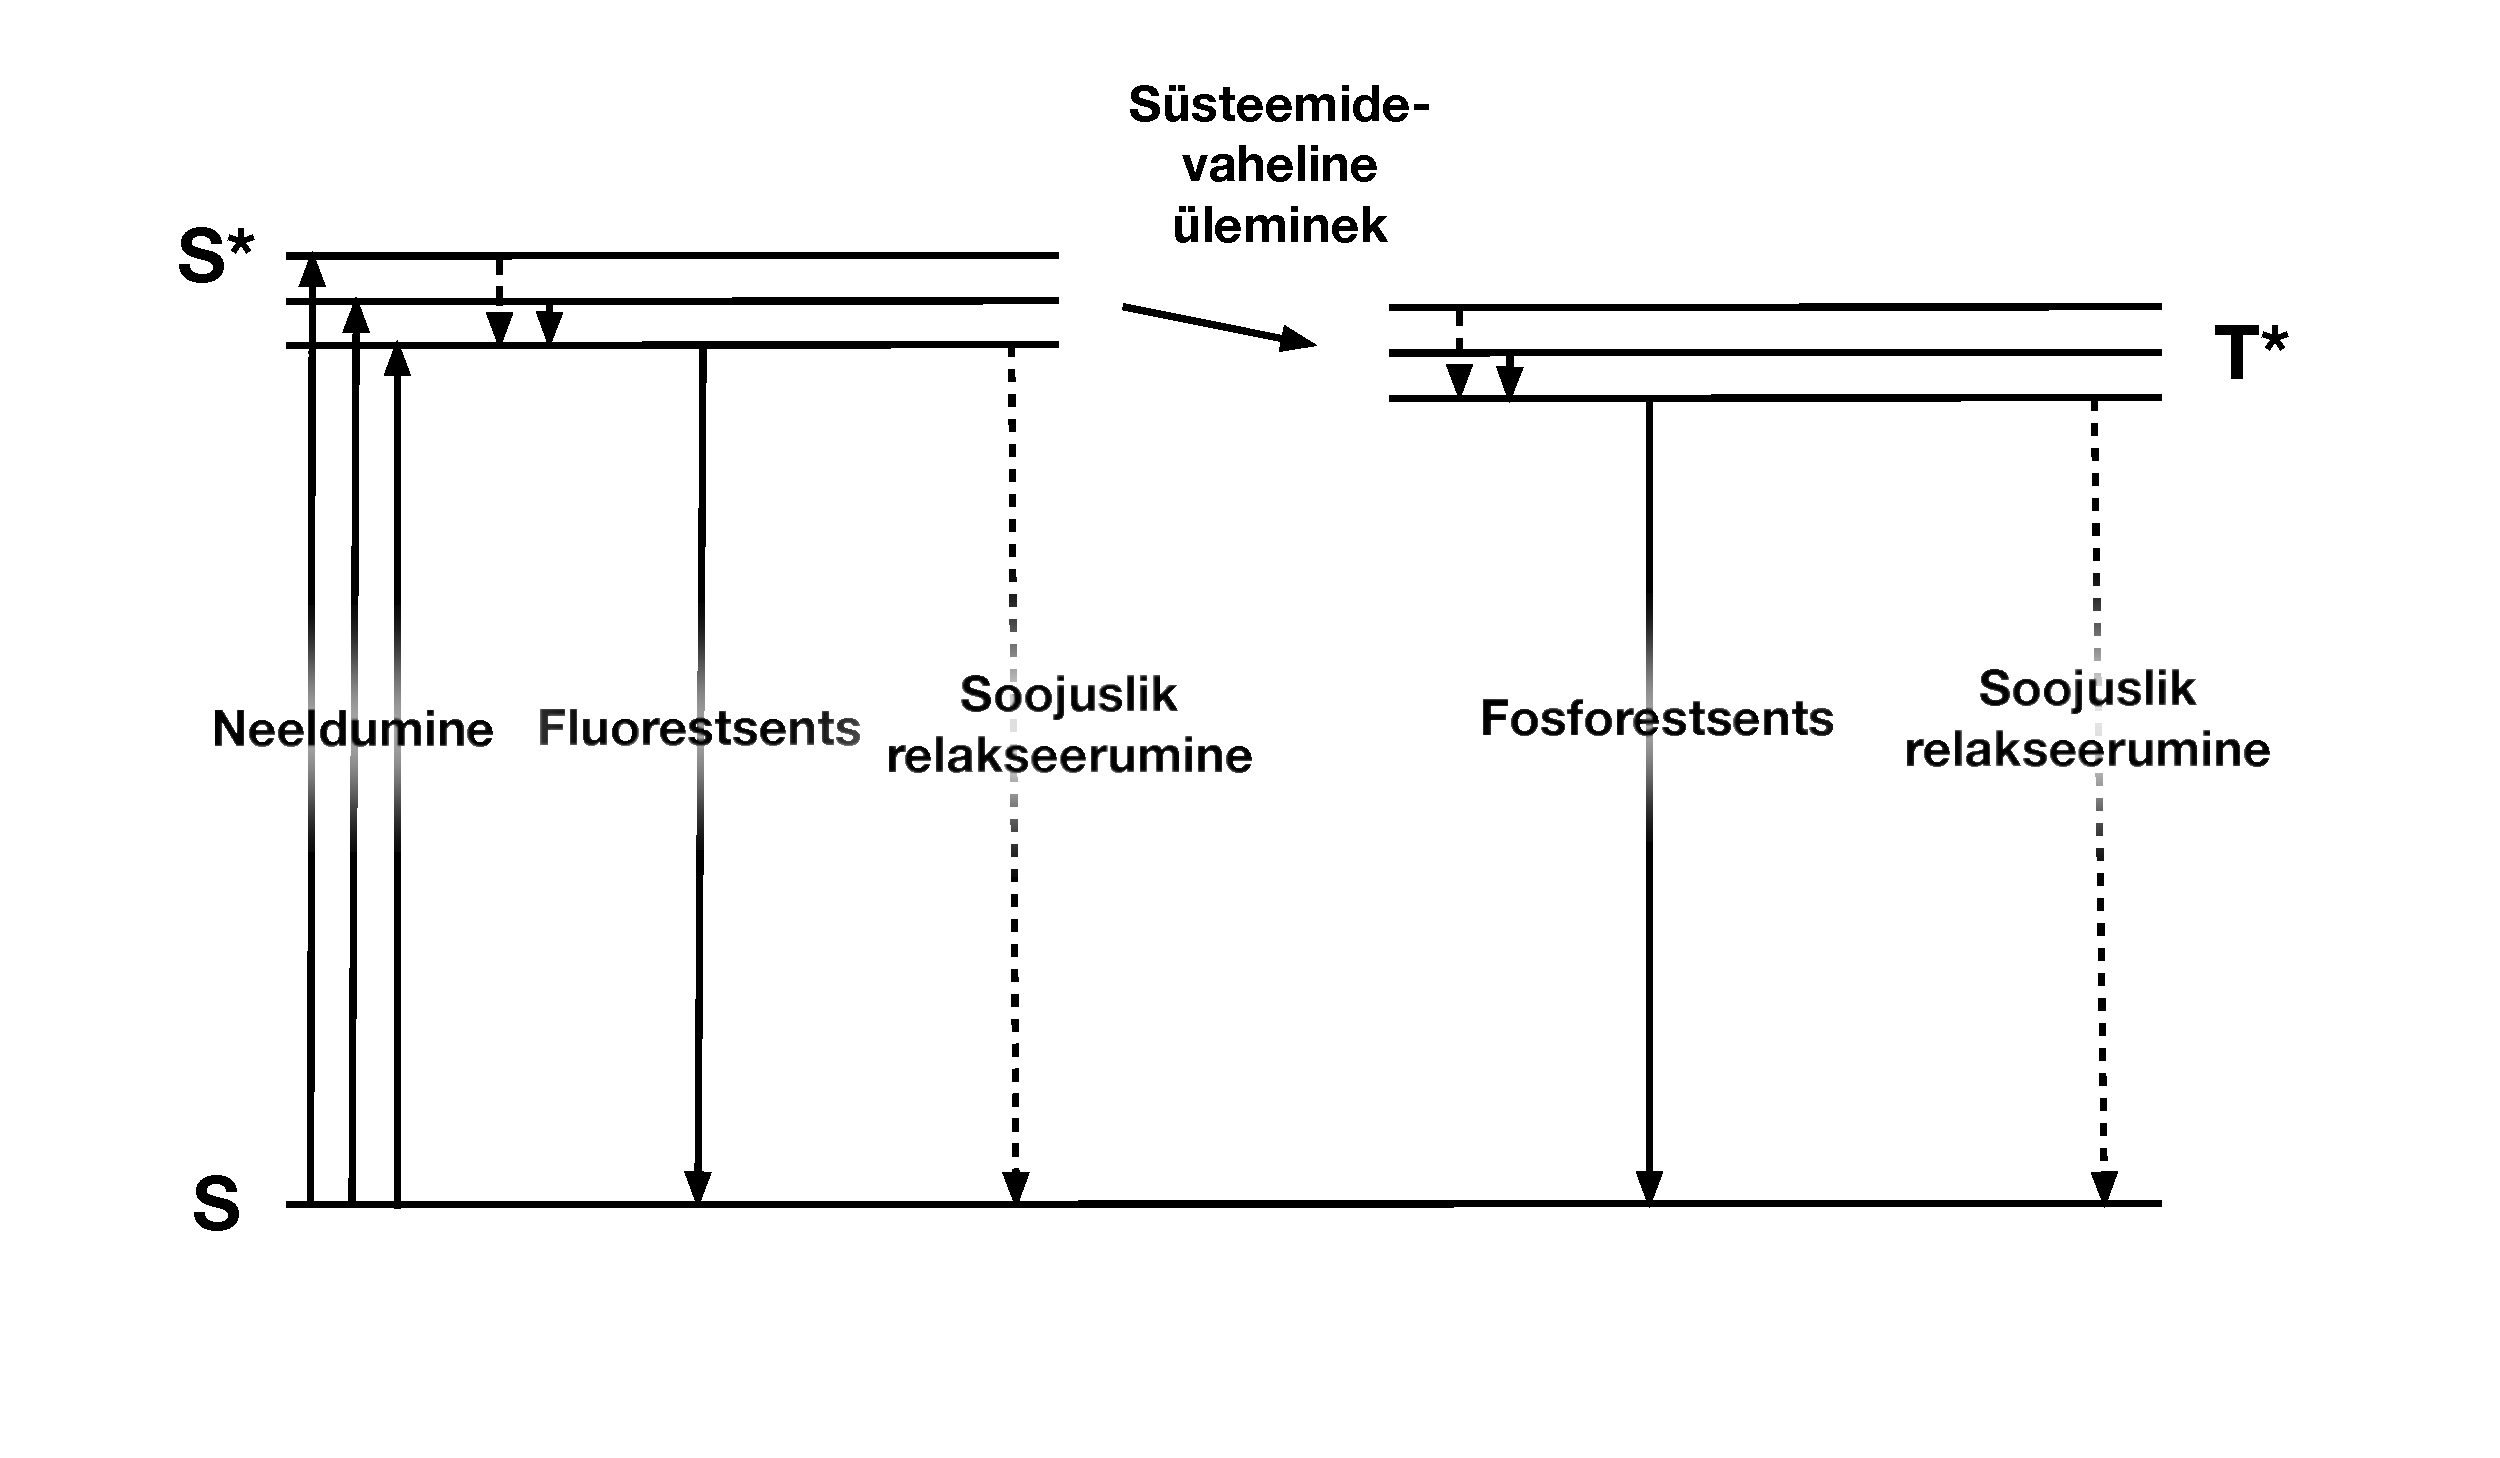
\includegraphics[width=\textwidth]{figures/jablonski.pdf}
    \caption{\label{jablonski}Lihtsustatud Jablonski diagramm. S vastab ühendi ergastamata põhiolekule, S$^*$ ja T$^*$ tähistavad vastavalt singletset ning tripletset ergastatud olekut. Punktiirjoonega on tähistatud mittekiirguslikud protsessid (nendega ei kaasne footoni neeldumist või eraldumist).}
\end{figure}

\subsection{Viitamine}

Viidata saab nii valemitele (vt valemeid \ref{gauss} ja \ref{gaussmagnet}), tabelitele (vaata tabel \ref{tabel}) kui ka joonistele (vt joonis \ref{jablonski}).

Viidata saab ka artiklitele \cite{iupac} ning raamatutele \cite{Atkins2005, Lakowicz2006}.
	
  %
% methods.tex
%
% Materjal ja metoodika
%

\section{Materjal ja metoodika}
	
  %
% results.tex
%
% Tulemused ja arutelu
%

\section{Tulemused ja arutelu}
	
  %
% summary.tex
%
% Kokkuvõte
%

\section{Kokkuvõte}

	%
% acknowledgements.tex
%
% Tänuavaldused
%

\section{Tänuavaldused}
	
	%
% summary_en.tex
%
% Inglisekeelne kokkuvõte
%

\section{Summary}

\subsection*{Title in English}
\subsubsection*{Author}
	
  \printbibliography

	%
% supplementary1.tex
%
% Lisa
%

\begin{appendices}

\section{Lisa}
\label{lisa1}

\end{appendices}
\end{document}
